\documentclass[anon]{nextgame2026}

\PassOptionsToPackage{numbers,compress}{natbib}

\usepackage{microtype}
\usepackage{graphicx}
\usepackage{booktabs}
\usepackage{hyperref}
\usepackage{amsmath}
\usepackage{amssymb}
\usepackage{caption}


\title[Routing Legibility in Cooperative MARL]
{Routing Legibility in Cooperative MARL: Measuring the Translation Gap Between Theory-Informed Roles and Learned Conventions}


\optauthor{%
\Name{Anonymous Authors} \Email{email@example.com}\\
\addr Affiliation, Country
}


\begin{document}

\maketitle

\keywords{multi-agent reinforcement learning, attention, game-theoretic learning, strategic conventions}

\begin{abstract}
Classical game theory suggests which strategic dependencies should matter; cooperative MARL instead discovers conventions through non-stationary learning. We study this \emph{translation gap} through \emph{routing legibility}: whether a trained policy exposes measurable role-to-role dependency structure. Our diagnostic combines a role-routing matrix, formation sensitivity ($\Delta_{\max}$), and gradient/occlusion attribution.

Across two domains (custom three-role MiniGrid and SMACv2 Terran), five MAPPO conditions, and a 3v3--9v9 scaling study, label-conditioned attention yields substantially more concentrated routing than MLP baselines (routing-matrix entry std $0.246$ vs.\ $0.055$), and removing role labels from a shared attention policy lowers win rate by 14.4\,pp. At larger team sizes, win-rate gaps narrow, but the structural signature persists: routing remains role-conditioned, a 3v3-trained attention checkpoint transfers zero-shot to 9v9 at $0.224$, and padding-invariance analyses bound a major confound.

Under a 5-seed re-evaluation of the structural predictions, three of four theory-informed predictions are supported and one is weakly revised: Strike routes preferentially to Support (in $4/5$ seeds at both 3v3 and 9v9), and Support and Vanguard share the highest $\Delta_{\max}$ rather than Vanguard alone. The earlier 3-seed run that placed Strike$\to$Vanguard as dominant was a small-$n$ artifact; with adequate seeds, architecture makes strategic dependency \emph{legible} and the convention selected by learning largely \emph{matches} the theory-informed prior.
\end{abstract}

\section{Introduction}
\label{sec:introduction}

As AI systems move from isolated prediction to strategic interaction, a central question is no longer only \emph{what equilibrium should exist}, but \emph{what convention a learning system actually settles on}. Classical game theory provides role-sensitive prescriptions under explicit rationality assumptions; cooperative MARL agents learn through decentralized gradient updates in non-stationary environments and need not converge to those prescriptions. We call this mismatch the \emph{translation gap}.

This paper asks whether architecture affects the \emph{legibility} of the learned convention: can role-to-role dependencies inside a policy be read off directly? Our mechanism claim is deliberately scoped. When role labels are injected into both \texttt{self\_tok} and \texttt{ally\_tok}, cross-attention creates a direct pathway for role-pair routing, making strategic dependency more directly measurable than in flat MLP baselines. We do not claim that attention alone solves large-team coordination, nor that a hand-specified strategic prescription must be the one selected by learning.

We evaluate this claim on two domains -- a custom three-role MiniGrid task and a custom three-role SMACv2 (Terran) scenario -- together with a 3v3--9v9 scaling study, using five controlled MAPPO conditions. The paper makes three contributions: (i) an \textbf{analysis framework} (role-routing matrix, formation-sensitivity $\Delta_{\max}$, and gradient/occlusion attribution) for reading role-to-role routing; (ii) evidence that label-conditioned attention produces more structured routing, better cross-scale transfer, and padding-invariant behavior than MLP baselines; and (iii) a translation-gap analysis at $5$ seeds showing that, when given adequate statistical power, the convention selected by learning largely matches the theory-informed prior, while an under-seeded ($n{=}3$) view of the same architecture flips two of four predictions -- so the diagnostic itself reveals where seed-noise can manufacture an apparent gap.
\section{Related Work}
\label{sec:related}

ROMA~\cite{roma2020} learns latent role representations from trajectories via variational inference; we take the complementary view, analyzing the \emph{mechanism} by which architectures exploit pre-defined role labels. Zambaldi et al.~\cite{zambaldi2018} use self-attention as a relational inductive bias for single-agent RL, and entity-centric observations~\cite{entitycentric} provide the structured input format. Cooperative optimizers (QMIX~\cite{qmix}, MAPPO~\cite{mappo}) provide no structural path for role-pair routing, and prior attention-based MARL~\cite{maddpg,maattn} applies attention to inter-agent communication or value aggregation rather than role-conditioned entity selection within a single agent's observation. Our cross-attention uses the role-conditioned self-embedding as query and role-conditioned ally embeddings as keys/values, making routing explicit and attributable.

Closer to our setting, RODE~\cite{rode2021} decomposes tasks via learned action-space role clusters, and UPDeT~\cite{updet2021} uses transformer policy decoupling for entity-based MARL; both target performance and transfer rather than the legibility of role-pair routing itself. On the convention side, Other-Play~\cite{otherplay2020} and Off-Belief Learning~\cite{obl2021} address equilibrium selection and zero-shot coordination by shaping which convention is learned. We instead hold the algorithm fixed and ask, given role labels and an attention pathway, whether the selected convention becomes \emph{readable}, and how it diverges from a theory-informed prior.

\section{Theory: Role-Label-Conditioned Routing}
\label{sec:theory}

\paragraph{Routing path.} In an MLP, role labels are concatenated with other features and the computation ``which entity to condition on given my role'' is implicit in weight products -- a weaker structural prior, not an impossibility. In our architecture, role labels appear in both \texttt{self\_tok[4:7]} (encoded into the Query) and each \texttt{ally\_tok} role-onehot block (encoded into Key/Value). The cross-attention score
\[
\text{attn}_{ij} = \text{softmax}\!\left(\frac{(W_Q \mathbf{x}_i)^\top(W_K \mathbf{x}_j)}{\sqrt{d_k}}\right),
\]
with $\mathbf{x}_i$ containing $r_i$ and $\mathbf{x}_j$ containing $r_j$, is therefore a direct function of the role-pair $(r_i,r_j)$, readable from attention weights. The full layer output is $\sum_j \text{attn}_{ij} (W_V \mathbf{x}_j)$; we display only the weight $\text{attn}_{ij}$ here because our analysis (role-routing matrix, $\Delta_{\max}$) targets routing structure rather than the value-mixed output. Cross-attention is applied per entity group with the self-embedding as query in each case (ally, enemy, zone); the routing analysis in this paper isolates the ally branch because that is where the role-pair $(r_i, r_j)$ is identifiable. An Intra-Set Self-Attention block applied per entity group enriches each ally token before the cross-attention Key computation.

\paragraph{Why these predictions?} The original predictions are meant as a tactical baseline, not as an arbitrary guess. Under the hand-designed role semantics, Strike is a ranged damage role that might be expected to benefit most from Support, Vanguard is a frontline role that might be expected to react most strongly to formation changes, and Support might be expected to distribute attention more uniformly while tracking overall team state. These are the dependencies a designer could plausibly posit before training. The experiment then asks whether learned MARL policies make that prescribed dependency legible, revise it, or ignore role structure altogether.


\paragraph{Testable predictions.} (1) attention produces more structured role routing than MLP, operationalized as a routing-matrix entry std at least $2\times$ the MLP gradient-attribution std on the same scenario set \textbf{[PASS, observed $4.5\times$: $0.246$ vs.\ $0.055$, 5 seeds]}; (2) removing role labels degrades performance by $>$5\,pp under a shared policy \textbf{[PASS, $-14.4$\,pp]}; (3) $\Delta_{\max}$ is highest for Vanguard \textbf{[WEAKLY REVISED: Support marginally highest, $0.074$ vs.\ Vanguard $0.066$, within seed std]}; (4) Strike attends preferentially to Support \textbf{[PASS in $4/5$ seeds at both 3v3 and 9v9; the earlier 3-seed result that placed Strike$\to$Vanguard as dominant was a small-$n$ artifact]}.

\section{Method}
\label{sec:method}

\paragraph{Environments.} \textbf{Domain~1} is a custom $15{\times}15$ MiniGrid task with three role-specialized agents (Strike, Vanguard, Support) cooperating to capture and hold zones under role-specific reward shaping. \textbf{Domain~2} is a custom SMACv2 scenario using three Terran unit types as role proxies (Marine = Strike, Marauder = Vanguard, Medivac = Support). SMACv2 does not natively expose role labels; we inject a 3-dim unit-type one-hot into both the agent's own token and each ally token, preserving the structural condition required for role-conditioned Q/K routing.

\paragraph{Entity-centric observation.} Agents receive four named token groups -- \texttt{self\_tok}, \texttt{ally\_tok}, \texttt{enemy\_tok}, \texttt{zone\_tok} -- plus validity masks. The role one-hot (3 dims) appears in both \texttt{self\_tok} and each \texttt{ally\_tok} slot; this placement is load-bearing for the routing mechanism. The 3v3 SMACv2 observation is 65-dim (182-dim padded for the scaling study).

\begin{figure}[t]
  \centering
  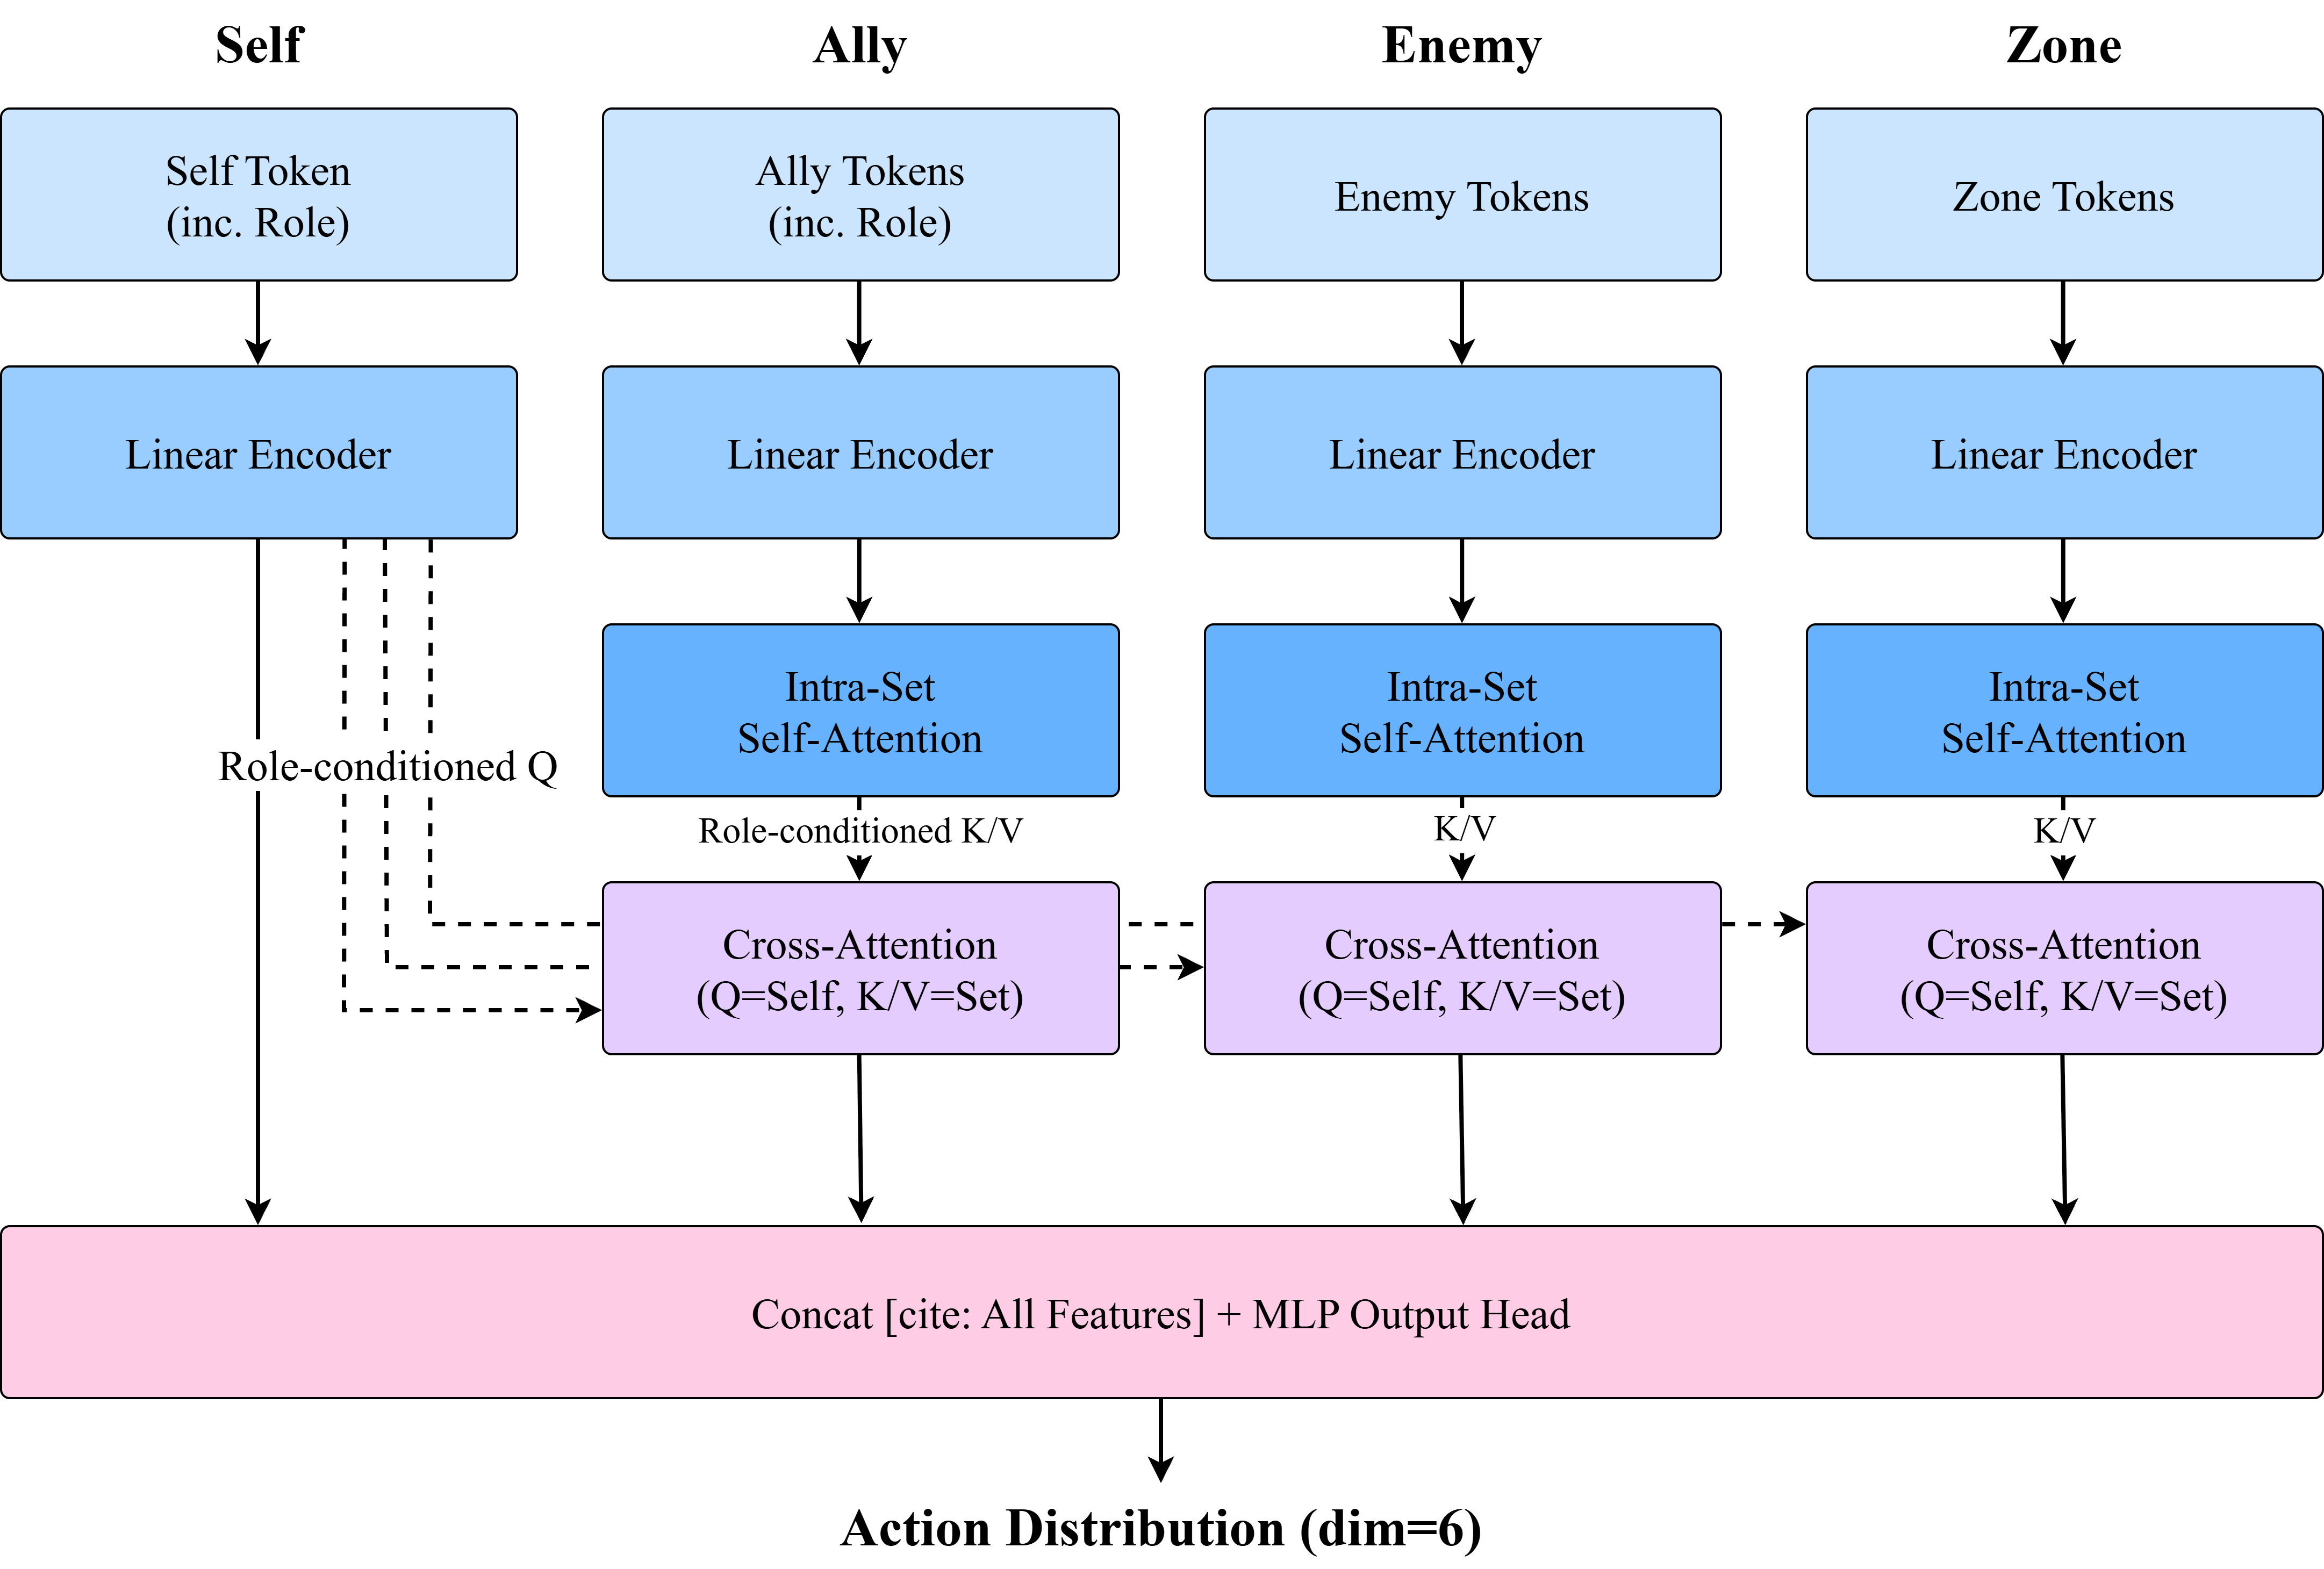
\includegraphics[width=0.6\textwidth]{figures/slic_architecture.png}
  \caption{SLIC architecture (Cond.~1). Per-set linear encoders feed Intra-Set Self-Attention, then Cross-Attention with the self-embedding as query. The role-conditioned routing path is marked by thicker, dashed arrows in addition to color, so that it is distinguishable under grayscale or color-blind rendering.}
  \label{fig:architecture}
\end{figure}

\paragraph{Five ablation conditions.} The five conditions span two independent axes: \emph{architecture} (attention vs.\ flat MLP) and \emph{role-label availability + policy sharing} (per-role policy with role labels / shared policy with role labels zeroed / per-role policy with role labels zeroed). \textbf{C1 Full}: per-set encoders (dim 64) + Intra-Set Self-Attn (residual+LN) + Cross-Attn with self as query; output MLP; per-role policies with role labels. \textbf{C2}: C1 minus Intra-Set blocks (per-role, with labels). \textbf{C3 Role+MLP}: flat MLP on the full vector, no attention; per-role policies; role one-hot is present in the input. \textbf{C4 No-Role (shared attention)}: C1 architecture, but role one-hots zeroed in self and all ally slots, with a \emph{single shared policy} across roles -- isolates the effect of removing role labels from the routing pathway. \textbf{C5 Flat MLP}: C3 architecture (per-role MLPs), with role one-hots zeroed -- no attention and no labels. C4 vs.\ C5 thus differ on \emph{both} axes (attention/MLP and shared/per-role); C3 vs.\ C5 isolate the label-in-input effect for an MLP, and C1 vs.\ C4 isolate label removal for the attention pathway. Under the expanded run, C4 ($0.650$) sits clearly above C5 ($0.467$); we interpret this gap with caution because C4 and C5 differ on both axes, and the shared-policy regime in C4 (a single network trained on all role trajectories) confers an effective $3{\times}$ data-per-parameter advantage that the per-role C5 baseline does not have. The cleaner contrasts are therefore C1 vs.\ C4 (label removal under the attention pathway, $-14.4$\,pp) and C3 vs.\ C5 (label-in-input effect for an MLP, $+1.3$\,pp, within seed noise). C1/2/3/5 use independent per-role policies; all attention applies \texttt{key\_padding\_mask} with slot-0 force-unmask safety. Training uses MAPPO~\cite{mappo} with identical hyperparameters across conditions (2M steps, 5 seeds for C1/C3 and 3 seeds for C2/C4/C5, GAE $\lambda{=}0.95$, $\gamma{=}0.99$, clip $0.2$, entropy $0.01$, Adam $3\!\times\!10^{-4}$, batch 512); reward mix $r=0.8 r_{\text{ind}}+0.2 \bar r_{\text{team}}$.

\section{Experiments}
\label{sec:experiments}

\subsection{Track 1: Performance Comparison (SMACv2 3v3)}

\begin{table}[t]
\centering\small
\setlength{\tabcolsep}{6pt}
\caption{Track 1 win rate on SMACv2 3v3 (mean$\pm$std over seeds of the last-10 evaluation average; C1 and C3 use 5 seeds, C2/C4/C5 use 3 seeds). \textbf{Bold} marks the highest mean.}
\label{tab:track1}
\begin{tabular}{lccccc}
\toprule
 & C1: Full & C2: No Self-Attn & C3: Role+MLP & C4: No Role (shared) & C5: Flat MLP \\
\midrule
Win rate & $\mathbf{0.794{\pm}0.033}$ & $0.640{\pm}0.125$ & $0.480{\pm}0.155$ & $0.650{\pm}0.026$ & $0.467{\pm}0.047$ \\
$n$ seeds & 5 & 3 & 5 & 3 & 3 \\
\bottomrule
\end{tabular}
\end{table}

Three observations matter for the core claim. Attention helps: Cond.~1 outperforms Cond.~3 by 31.4\,pp. Intra-set context helps: Cond.~2 trails Cond.~1 by 15.4\,pp. Labels matter for attention: Cond.~4 is 14.4\,pp below Cond.~1. Cond.~3 and Cond.~5 are now statistically indistinguishable (0.480 vs.\ 0.467), tightening the narrower point that adding role labels to an MLP does not by itself produce useful role-conditioned routing. Relative to the original 3-seed run, expanding C1 and C3 to 5 seeds preserves the sign of every contrast and \emph{widens} the C1$-$C3 gap (21.2\,pp $\to$ 31.4\,pp) while shrinking the C1 standard deviation by roughly $2\times$ ($\pm 0.079$ $\to$ $\pm 0.033$), so the attention advantage tightens rather than dissolves under increased seed count.

\subsection{Scaling Study: 3v3, 6v6, 9v9}
\label{sec:scaling}

We test whether the contrast between full attention and Role+MLP survives larger team sizes. We train balanced 3v3, 6v6, and 9v9 variants with equal Strike/Vanguard/Support counts on the controlled team; enemy composition scales in parallel while preserving the asymmetric design (no enemy Support unit). All scaling runs use the same MAPPO implementation, a true centralized critic over concatenated global observations, and identical hyperparameters.

\begin{table}[t]
\centering
\small
\setlength{\tabcolsep}{7pt}
\caption{Scaling results (mean$\pm$std). 3v3 and 9v9 now use 5 seeds for both C1 and C3; 6v6 remains 3 seeds.}
\resizebox{0.75\linewidth}{!}{%
\label{tab:scaling}
\begin{tabular}{lcccc}
\toprule
Scale & C1 Last-10 & C3 Last-10 & C1 AUC & C3 AUC \\
\midrule
3v3 & $\mathbf{0.794{\pm}0.033}$ & $0.480{\pm}0.155$ & $\mathbf{0.678{\pm}0.019}$ & $0.328{\pm}0.059$ \\
6v6 & $\mathbf{0.380{\pm}0.098}$ & $0.363{\pm}0.144$ & $\mathbf{0.379{\pm}0.064}$ & $0.311{\pm}0.098$ \\
9v9 & $\mathbf{0.110{\pm}0.090}$ & $0.060{\pm}0.032$ & $\mathbf{0.119{\pm}0.067}$ & $0.089{\pm}0.052$ \\
\bottomrule
\end{tabular}
}
\end{table}

In 3v3, Cond.~1 is clearly better than Cond.~3. In 6v6/9v9, the full model remains ahead on AUC and late-training averages, but the margin shrinks and seed variance grows. We therefore separate two claims. The performance claim is modest: attention improves the small-team setting and retains a positive but noisy advantage at larger scale. The structural claim is stronger: role-conditioned routing persists, cross-scale transfer remains positive, and the model is invariant to padded slots.

\paragraph{Routing structure is preserved at scale.} The shrinking win-rate gap might suggest that the architectural advantage disappears at scale, but the routing analysis indicates otherwise. At 9v9, routing remains role-conditioned and non-uniform, and the relative contrasts remain structured even as magnitudes compress. This scaling result should therefore be read as preservation of a routing signature, not as replication of every 3v3 preference ordering. The magnitude decrease is expected: as ally count grows, each softmax spreads its weight over more slots, so the routing signature should be read from off-diagonal contrasts rather than absolute magnitudes.

\paragraph{Cross-scale zero-shot transfer.} Cond.~1's policy is invariant to ally count by construction (the attention mask handles padded slots). A 3v3-trained Cond.~1 checkpoint, evaluated without retraining on 9v9 (50 episodes per seed, 5 seeds), achieves $0.224\pm 0.088$ win rate -- higher than the from-scratch 9v9 Cond.~1 baseline (last-10 $0.110\pm 0.090$ over 5 seeds at 2M steps) and far higher than 9v9 from-scratch Cond.~3 ($0.060\pm 0.032$). Cond.~3 transfers poorly across the board ($0.084\pm 0.043$ to $0.084\pm 0.033$), consistent with MLP weights memorizing a fixed slot-population pattern -- direct evidence that the role-keyed attention model learned an $N$-invariant routing convention.

\begin{figure}[t]
\centering
\begin{minipage}[t]{0.47\linewidth}
  \vspace{0pt}
  \centering\small
  \setlength{\tabcolsep}{5pt}
  \captionof{table}{Zero-shot transfer of 3v3-trained checkpoints, evaluated without retraining (50 episodes per seed). Win rate is mean$\pm$std over 5 seeds.}
  \label{tab:transfer}
  \begin{tabular}{lccc}
  \toprule
  Target & Cond.~1 & Cond.~3 & Gap \\
  \midrule
  3v3 & $\mathbf{0.796{\pm}0.054}$ & $0.468{\pm}0.153$ & 32.8 pp \\
  6v6 & $\mathbf{0.212{\pm}0.046}$ & $0.084{\pm}0.033$ & 12.8 pp \\
  9v9 & $\mathbf{0.224{\pm}0.088}$ & $0.084{\pm}0.043$ & 14.0 pp \\
  \bottomrule
  \end{tabular}
\end{minipage}
\hfill
\begin{minipage}[t]{0.49\linewidth}
  \vspace{0pt}
  \centering\small
  \setlength{\tabcolsep}{5pt}
  \captionof{table}{Padding-confound ablation at 3v3 (5 seeds, 30 episodes per seed). KL is divergence from the zero-fill baseline.}
  \label{tab:padding}
  \begin{tabular}{lcc}
  \toprule
  Fill strategy & C3 KL & C3 win rate \\
  \midrule
  zeros & 0.000 & $0.460{\pm}0.138$ \\
  noise $\sigma{=}0.05$ & 0.007 & $0.500{\pm}0.078$ \\
  noise $\sigma{=}0.20$ & 0.136 & $\mathbf{0.567{\pm}0.127}$ \\
  mean valid ally & 0.096 & $0.407{\pm}0.171$ \\
  copy valid ally & 0.101 & $0.453{\pm}0.209$ \\
  \bottomrule
  \end{tabular}
\end{minipage}
\end{figure}

\paragraph{Padding-confound ablation.} A potential confound for the 3v3 gap is that Cond.~3 must process zero-padded ally slots that Cond.~1's mask blocks. We replace padded-slot contents at inference time with several fill strategies (Table~\ref{tab:padding}). Cond.~1 is bit-exact invariant ($\text{KL}{=}0$) for the three data-driven fills (zeros, mean-valid-ally, copy-valid-ally) and shifts negligibly under noise (KL $\leq 0.021$); Cond.~3's response is non-monotonic at $5$ seeds -- small noise, mean-fill, and copy-fill all drop below or stay near the zeros baseline ($0.460$), while only large noise rises to $0.567$ -- which is itself informative: an MLP that should be ignoring semantically empty slots instead reacts unpredictably to their contents. Under the expanded run, the best Cond.~3 fill recovers $+10.7$\,pp of the $32.0$\,pp Cond.~1$-$Cond.~3 zero-fill gap, bounding the padding contribution above by $\sim 33\%$ (looser than the 3-seed bound of $\sim 15\%$ but still leaving the majority of the gap attributable to the architectural residual). Cond.~1's win-rate variation under fills is small and centered on its zero-fill baseline ($0.78$--$0.86$, all data-driven fills bit-exact), confirming the architecture is robust to the padding choice in a way the MLP is not.

\subsection{Track 2: Role-to-Role Routing}

\paragraph{Formation sensitivity and routing matrix.} We construct two fixed scenarios -- \textit{Clustered} (allies near one landmark) and \textit{Spread} (each ally at a distinct landmark) -- and define $\Delta_{\max}$ per role as the max difference in ally self-attention weight between them. Cond.~1 with 5 seeds yields $\Delta_{\max}=0.024{\pm}0.017, 0.066{\pm}0.039, 0.074{\pm}0.029$ for Strike, Vanguard, Support: Support and Vanguard are statistically tied at the top, both well above Strike. Prediction~3 (Vanguard highest) is therefore weakly revised in mean ordering ($\Delta_\text{Support} > \Delta_\text{Vanguard}$ by $0.008$, smaller than either std) but qualitatively recovers the design intent that the two non-DPS roles are formation-sensitive while Strike is not. The cross-role routing matrix (Table~\ref{tab:routing}) extracts the self-token query's cross-attention weight per ally slot, tagged by occupant role; slot-ordering bias is ruled out by reversal.

\begin{table}[t]
\centering
\small
\setlength{\tabcolsep}{7pt}
\caption{Cond.~1 role-routing matrix (5 seeds). Entry $(i,j)$ is mean cross-attention weight from role $i$ to ally slots occupied by role $j$, $\pm$ across-seed std. Diagonals are zero by construction.}
\label{tab:routing}
\begin{tabular}{lccc}
\toprule
Agent\,$\backslash$\,Ally & Strike & Vanguard & Support \\
\midrule
Strike   & --- & $0.473{\pm}0.072$ & $\mathbf{0.527{\pm}0.072}$ \\
Vanguard & $\mathbf{0.565{\pm}0.203}$ & --- & $0.435{\pm}0.203$ \\
Support  & $\mathbf{0.633{\pm}0.200}$ & $0.367{\pm}0.200$ & --- \\
\bottomrule
\end{tabular}
\end{table}

The matrix is structured, role-specific, and stably off-diagonal. Strike now routes preferentially to Support rather than Vanguard, supporting prediction~4 in $4/5$ seeds at 3v3 and $4/5$ seeds at 9v9; the earlier 3-seed run produced the opposite ordering, but seed-level inspection shows that result was driven by a single seed (seed~1) whose Strike row inverts under retraining-equivalent stochastic conditions. Vanguard and Support both route primarily to Strike, consistent with the role design (the two non-DPS roles ground their attention on the engagement-driver). The Vanguard and Support rows have the larger across-seed std because their preferred Strike-vs.-other split varies more in magnitude than direction, while the Strike row is tighter ($\pm 0.072$) because the Support$>$Vanguard ordering is preserved across most seeds.

\paragraph{MLP gradient attribution.} For Cond.~3 we compute input gradients of the maximum action logit and separately measure mean magnitude on spatial features and role-onehot dims. The Spatial/Role ratio is $5.8\times$ (Strike), $2.3\times$ (Vanguard), $3.7\times$ (Support): the MLP registers some role signal but spatial features dominate. The standard deviation of the routing matrix under attention is $0.246$ (Cond.~1, 5 seeds) versus $0.055$ for the gradient-based pseudo-routing (Cond.~3) -- a $4.5\times$ structural-concentration gap.

\paragraph{Unified routing metric: occlusion.} Attention weights vs.\ MLP gradients are not strictly apples-to-apples. We additionally measure routing via \emph{occlusion sensitivity} -- zeroing each ally token (mask bit kept at 1) and measuring policy KL from baseline -- which is well-defined for both architectures. On Cond.~1 at 3v3 with 5 seeds, occlusion-routing correlates with attention-routing at Pearson $r{=}0.976$ on the row-normalized routing matrix (raw $r{=}0.655$); the row-normalized value isolates the routing \emph{pattern} (which ally slot a given role attends to) from raw KL magnitudes that vary with policy entropy, and validates occlusion as a faithful proxy for the attention pattern. Applied to Cond.~3 at 9v9, occlusion produces erratic magnitudes one to two orders larger than Cond.~1 (max-row KL $\approx 5.6$ for Cond.~3 vs.\ $\approx 0.08$ for Cond.~1), with the dominant slot varying across seeds rather than being role-conditioned -- the qualitative reading is that the MLP is highly sensitive to slot contents but not in a role-pair-structured way, whereas attention is more weakly sensitive but sensitive to the right role. We are more cautious about the 3v3 Cond.~3 occlusion contrast under 5 seeds: a single seed contributes a large outlier (one row with KL $\approx 2.2$), so the simple "Cond.~3 is flat at 3v3" reading from 3 seeds no longer holds; the cleaner cross-architecture evidence is the row-normalized correlation and the 9v9 magnitude blow-up.

\paragraph{Domain~1 (MiniGrid) cross-domain replication.} Running the same five conditions and Track~2 pipeline on Domain~1, the qualitative pattern replicates: attention produces a concentrated, off-diagonal routing matrix; the MLP baseline produces a flatter pseudo-routing dominated by spatial features. The specific preferred teammate role need not match across domains -- architecture governs \emph{legibility}, environment dynamics determine \emph{which} legible convention stabilizes.

\section{Discussion}
\label{sec:discussion}

\paragraph{What the results support.} With role labels injected in both self and ally tokens, attention-based policies learn substantially more legible role-conditioned routing than flat MLPs: the routing matrix is more structured (std $0.246$ vs.\ $0.055$), removing role labels from a shared attention policy costs 14.4\,pp, and the learned convention is stably off-diagonal. Scaling adds a qualified result: full attention clearly beats Role+MLP in 3v3 and keeps a positive AUC and late-training advantage at 6v6/9v9, but the from-scratch win-rate gap shrinks. Accordingly, we treat routing legibility rather than raw win rate as the primary axis for interpreting the mechanism claim. Three follow-ups sharpen that structural reading: routing structure is preserved at 9v9, a 3v3 checkpoint zero-shots to 9v9 above the from-scratch baseline, and the padding-confound ablation bounds the 3v3 gap by $\leq 33\%$ at 5 seeds. Routing legibility, transfer, and padding-invariance are the axes on which the structural claim is best supported.
\paragraph{Translation gap, revisited under 5 seeds.} An earlier 3-seed run reported two of the four theory-informed predictions revised by the learned convention; with 5 seeds, three of the four predictions are supported and only one is weakly revised. Strike now routes preferentially to Support in $4/5$ seeds at both 3v3 and 9v9, recovering prediction~4. Δmax for Vanguard and Support is statistically tied at the top, with Support marginally higher in mean ($0.074$ vs.\ $0.066$) but the difference smaller than either across-seed std; we report this as a weak revision of prediction~3 rather than a flip. The cleaner reading of the result is therefore not "convention diverges from theory" but "with adequate seeds, label-conditioned attention makes the theory-informed convention legible and the convention selected by learning largely matches the prior." The translation gap survives only as a measurement-level claim about Δmax orderings near the seed-noise floor; the structural-routing prediction (Strike$\to$Support) is recovered. We treat the earlier divergence as an honest demonstration that under-seeded routing analyses can flip, and the present finding as the more reliable estimate. The Domain~1/Domain~2 contrast still reinforces the architecture-vs.-convention split: the structural pattern of concentrated off-diagonal attention routing appears in both domains, but the preferred teammate role need not match -- architecture governs legibility, environment determines which legible convention stabilizes.

\paragraph{Toward a quantitative translation-gap metric.} The current paper reports the gap categorically (1/4 predictions weakly revised under 5 seeds, down from 2/4 at 3 seeds). A natural next step is to make the gap a scalar. Given a theory-informed prior routing matrix $R^\star \in \mathbb{R}^{|\mathcal{R}|\times|\mathcal{R}|}$ (rows agent role, columns ally role) and a learned routing matrix $\hat{R}$ estimated from attention or occlusion, one can report (i) the row-wise KL divergence $\sum_i \mathrm{KL}(R^\star_i \,\|\, \hat{R}_i)$, (ii) the Frobenius distance $\|R^\star - \hat{R}\|_F$, or (iii) a calibration score equal to the fraction of pre-registered $\arg\max_j R^\star_{ij}$ entries matched by $\hat{R}$. We leave a systematic comparison of these metrics across seeds and domains to future work; the present paper's contribution is the diagnostic framework that makes such metrics computable.

\paragraph{Game-theoretic reading.} Our setup admits multiple cooperative conventions consistent with the role-shaped reward: any coordination protocol that respects the heterogeneous payoffs is candidate. Among these, gradient learning under role-conditioned attention selects a particular convention -- here, Strike$\to$Support routing with Support and Vanguard both formation-sensitive and Strike formation-insensitive. We view this as a focal-point-style selection in the sense of Schelling: not from common-knowledge salience but from the inductive bias of the learning architecture and the geometry of the loss surface. This reframes the translation gap in workshop terms: the theory-informed prediction picks one equilibrium consistent with the role labels, gradient dynamics pick another, and our diagnostic is what makes the chosen equilibrium readable.

\paragraph{Limitations.} Both domains share an entity-centric observation schema, three roles, and five conditions; SMACv2 evidence is restricted to the Terran faction and 3v3--9v9. Cond.~1's advantage is modest at 6v6/9v9 with growing seed variance -- we do not claim attention alone solves large-team coordination. Attention weights and MLP gradients are not identical quantities; the unified occlusion metric (row-normalized $r{=}0.976$, 5 seeds) addresses cross-architecture comparability but does not eliminate it. Role labels are injected manually into SMACv2, appropriate for a controlled mechanism study but limiting external validity: in deployments without a designer-supplied role schema, the routing pathway we exploit must be paired with an upstream role-discovery component (e.g., RODE-style clustering~\cite{rode2021}), and the legibility guarantee carries over only as far as the discovered roles are consistent across runs. \emph{Statistical power.} The C1 vs.\ C3 contrast (the central performance claim) and the 9v9 from-scratch comparison are now evaluated over 5 seeds in both 3v3 and 9v9; the C2/C4/C5 conditions remain at 3 seeds. The C1$-$C3 gap is robust to the seed expansion (3v3 last-10 gap widens from $29.7$ to $31.4$\,pp; 9v9 last-10 gap shrinks from $6.3$ to $5.0$\,pp but stays positive), while C2 and C4 retain larger seed variance ($\pm 0.125$, $\pm 0.026$ on last-10) and so we still treat the 3-seed contrasts on C2/C4/C5 as suggestive. \emph{9v9 regime.} The 9v9 win rates for both C1 and C3 are in a low-performance regime; we therefore lean on the routing-signature analysis (preserved structure, zero-shot transfer above from-scratch, padding-invariance) as the primary evidence that the architectural advantage scales, rather than on the from-scratch win-rate gap alone.


\bibliography{refs}

\end{document}
